\documentclass[11pt]{article}

\usepackage[margin=1in]{geometry}
\usepackage{amsmath,amsthm,amssymb,amsfonts}
\usepackage{hyperref}
\usepackage{tikz-cd}    % for commutative diagrams
\usepackage{pgfplots}   % for the example figure using 'axis' environment
\pgfplotsset{compat=1.17}

\newtheorem{definition}{Definition}[section]
\newtheorem{theorem}{Theorem}[section]
\newtheorem{lemma}{Lemma}[section]
\newtheorem{proposition}{Proposition}[section]
\newtheorem{corollary}{Corollary}[section]
\newtheorem{remark}{Remark}[section]
\newtheorem{example}{Example}[section]

\title{\textbf{A Unification of Linguistics and Spectral Theory via the Functorial Fourier Transform and Universal Linguistic Functor}}
\author{
  \textbf{Matthew Long}\\
  \textit{Magneton Labs}
}
\date{\today}

\begin{document}

\maketitle

\begin{abstract}
We introduce a novel, highly theoretical framework for a \emph{functorial Fourier transform} in the category \(\mathbf{Gram}\) of formal grammars, driven by a universal linguistic functor \(\mathcal{F}\). By embedding grammars in appropriate Hilbert spaces and invoking a generalized Fourier operator, we demonstrate how this construction can yield new insights into the compositional and spectral properties of language. We present the underlying categorical concepts, prove key theorems about the existence and naturality of the Fourier transform as a critical operator, and discuss potential ramifications for both formal language theory and abstract approaches to linguistics. 

We additionally illustrate how \emph{Fast Fourier Transform (FFT)} ideas can manifest in grammatical derivations, show a concrete example with a simple grammar, and highlight applications to grammar induction, quantum parsing algorithms, and non-commutative extensions.
\end{abstract}

\tableofcontents

\section{Introduction}

Modern linguistic and computational frameworks rely heavily on formal grammars as foundational objects. Simultaneously, harmonic analysis and the Fourier transform have proven indispensable in a vast range of mathematical and engineering fields, from classical signal processing to quantum mechanics. In this paper, we propose a unifying theoretical perspective in which \textbf{the Fourier transform} is conceptualized as a \emph{functorial} construction over the category \(\mathbf{Gram}\) of grammars, linked by a \emph{universal linguistic functor} \(\mathcal{F}\). 

We believe that bridging grammatical structure with Fourier-theoretic perspectives can:
\begin{itemize}
    \item Illuminate inherent ``spectral signatures'' of derivational processes in a grammar.
    \item Provide a unified language of compositional structure that is compatible with both syntactic and semantic interpretations.
    \item Facilitate deeper connections between symbolic and analytic methods, potentially impacting fields like formal language theory, computational linguistics, and even quantum linguistic models.
\end{itemize}

\paragraph{Main Contributions.}
\begin{enumerate}
    \item \textbf{Category \(\mathbf{Gram}\)}: We outline the categorical structure of grammars and grammar morphisms, including relevant subcategories for context-free and other grammar classes.
    \item \textbf{Universal Linguistic Functor \(\mathcal{F}\)}: We define \(\mathcal{F} : \mathbf{Gram} \to \mathbf{Hilb}\), showing how each grammar is mapped to a suitable Hilbert space based on derivations.
    \item \textbf{Functorial Fourier Transform}: We construct the operator \(\mathsf{FT}_G\) for each grammar \(G\), prove its functorial properties, and show that the collection of these operators can be organized as a natural transformation.
    \item \textbf{FFT-like Methods and Applications}: We extend the functorial transform to exploit recursive grammar structures, discuss the analogy to classical FFT, and demonstrate applications to grammar induction and quantum parsing.
\end{enumerate}

\section{Preliminaries}

\subsection{Categories and Functors}

We assume familiarity with the basics of category theory (see \cite{maclane} for a comprehensive reference). Recall:
\begin{itemize}
    \item A \emph{category} \(\mathbf{C}\) consists of objects and morphisms satisfying associativity and identity axioms.
    \item A \emph{functor} \(F : \mathbf{C} \to \mathbf{D}\) sends each object and morphism in \(\mathbf{C}\) to an object and morphism in \(\mathbf{D}\) in a structure-preserving way.
    \item A \emph{natural transformation} \(\eta : F \Rightarrow G\) between functors \(F, G : \mathbf{C} \to \mathbf{D}\) consists of components \(\eta_X : F(X) \to G(X)\) for each object \(X\in \mathbf{C}\), commuting with all morphisms of \(\mathbf{C}\).
\end{itemize}

\subsection{Fourier Analysis in Hilbert Spaces}

Let \(\mathcal{H}\) be a Hilbert space over \(\mathbb{C}\). A \emph{Fourier transform} is typically an isometric isomorphism from one function space (e.g.\ \(L^2\) of some domain) to another (e.g.\ its dual domain). We will use the term ``Fourier transform'' in a generalized sense, referring to an operator \(\mathsf{FT}\) that diagonalizes or decomposes a function-like object into an appropriate ``frequency-like'' basis. Classical references include \cite{folland}.

\section{The Category \texorpdfstring{\(\mathbf{Gram}\)}{Gram}}

\begin{definition}[Category \(\mathbf{Gram}\)]
Let \(\mathbf{Gram}\) be the category where:
\begin{itemize}
    \item \textbf{Objects} are formal grammars \(G\), together with their derivations \(\mathcal{D}(G)\).
    \item \textbf{Morphisms} \(\alpha : G_1 \to G_2\) preserve the grammatical structure, mapping derivations in \(\mathcal{D}(G_1)\) to valid derivations in \(\mathcal{D}(G_2)\).
\end{itemize}
\end{definition}

Depending on context, \(\mathbf{Gram}\) may be restricted to context-free grammars, type-0 grammars, or more specialized classes. One may also consider \(\mathbf{Gram}\) to be a 2-category or bicategory if we track transformations between grammar morphisms (translations, expansions, etc.).

\subsection{Examples}

\begin{example}[Context-Free Grammars]
Let \(\mathbf{CFG}\) be the subcategory where each object is a context-free grammar specified by \((V, \Sigma, R, S)\), and morphisms are grammar homomorphisms preserving production rules. \(\mathbf{CFG}\) includes classical constructions like pushdown automata.
\end{example}

\section{Universal Linguistic Functor}

\begin{definition}[Universal Linguistic Functor \(\mathcal{F}\)]
A functor \(\mathcal{F}: \mathbf{Gram} \to \mathbf{Hilb}\) is said to be \emph{universal linguistic} if it satisfies:
\begin{enumerate}
    \item For each grammar \(G\in\mathbf{Gram}\), \(\mathcal{F}(G) = \mathcal{H}_G\) is a Hilbert space constructed from \(\mathcal{D}(G)\) (e.g.\ spanned by basis vectors or wavefunctions indexed by derivations).
    \item For each morphism \(\alpha: G_1 \to G_2\), \(\mathcal{F}(\alpha) : \mathcal{H}_{G_1} \to \mathcal{H}_{G_2}\) is a bounded linear map respecting the compositional structure of derivations.
    \item \(\mathcal{F}\) is \emph{fully faithful} with respect to relevant substructures of \(\mathbf{Gram}\), ensuring minimality or maximality conditions (depending on the chosen universal property).
\end{enumerate}
\end{definition}

The construction of \(\mathcal{H}_G\) might be approached in several ways:
\begin{itemize}
    \item \emph{Orthogonal basis of derivations}: each derivation \(d \in \mathcal{D}(G)\) becomes a basis vector \(\lvert d \rangle\).
    \item \emph{Weighted spaces}: assign measures or probabilities to derivations, forming \(L^2\)-type spaces.
    \item \emph{Operator algebras}: interpret grammar production rules as operators in \(\mathcal{H}_G\).
\end{itemize}

\section{The Functorial Fourier Transform}

We now introduce our primary object of study: a \emph{Fourier transform operator} \(\mathsf{FT}_G\) for each grammar \(G\), assembled into a natural transformation of functors. 

\begin{definition}[Functorial Fourier Transform Operator]
For a grammar \(G\in \mathbf{Gram}\), let \(\mathsf{FT}_G : \mathcal{H}_G \to \mathcal{H}_G\) be a linear (preferably unitary) operator. We say these operators \(\{\mathsf{FT}_G\}\) form a \emph{functorial Fourier transform} if for every morphism \(\alpha: G_1 \to G_2\) in \(\mathbf{Gram}\), the following diagram commutes:
\[
\begin{tikzcd}
\mathcal{H}_{G_1} \arrow[r, "\mathcal{F}(\alpha)"] \arrow[d, "\mathsf{FT}_{G_1}"']
& \mathcal{H}_{G_2} \arrow[d, "\mathsf{FT}_{G_2}"] \\
\mathcal{H}_{G_1} \arrow[r, "\mathcal{F}(\alpha)"']
& \mathcal{H}_{G_2}
\end{tikzcd}
\]
That is, 
\[
\mathcal{F}(\alpha) \circ \mathsf{FT}_{G_1} \;=\; \mathsf{FT}_{G_2} \circ \mathcal{F}(\alpha).
\]
\end{definition}

Equivalently, this means that the assignment \(G \mapsto \mathsf{FT}_G\) is a \emph{natural transformation} from \(\mathcal{F}\) to \(\mathcal{F}\).

\subsection{Discrete vs.~Continuous Fourier}

\begin{itemize}
\item \emph{Discrete setting:} If \(\mathcal{D}(G)\) is finite or countably infinite, one may define a discrete Fourier transform (DFT) by interpreting the indexing set as a finite group or a direct sum of cyclic groups.
\item \emph{Continuous setting:} If derivations in \(\mathcal{D}(G)\) can be parameterized by a continuous domain (or have measure-theoretic structure), one can adopt an \(L^2\) Fourier transform on \(\mathbb{R}^n\) or more general groups.
\end{itemize}

\section{Main Results}

\subsection{Existence and Uniqueness under Mild Hypotheses}

\begin{theorem}[Existence of a Functorial Fourier Transform]
\label{thm:existence-fft}
Suppose \(\mathcal{F}: \mathbf{Gram} \to \mathbf{Hilb}\) is a universal linguistic functor such that for every grammar \(G\), the space \(\mathcal{H}_G\) has a well-defined group-like or measure-theoretic structure on \(\mathcal{D}(G)\). Then there exists a collection \(\{\mathsf{FT}_G\}_{G \in \mathbf{Gram}}\) of linear (or unitary) operators making the following diagram commute for all morphisms \(\alpha\):
\[
\begin{tikzcd}
\mathcal{H}_{G_1} \arrow[r, "\mathcal{F}(\alpha)"] \arrow[d, "\mathsf{FT}_{G_1}"']
& \mathcal{H}_{G_2} \arrow[d, "\mathsf{FT}_{G_2}"] \\
\mathcal{H}_{G_1} \arrow[r, "\mathcal{F}(\alpha)"']
& \mathcal{H}_{G_2}
\end{tikzcd}
\]
In other words, \(\{\mathsf{FT}_G\}\) defines a natural transformation \(\widehat{(\cdot)} : \mathcal{F} \Rightarrow \mathcal{F}\).
\end{theorem}

\begin{proof}[Sketch of Proof]
\noindent
\textbf{Step 1 (Discrete Base Case).}  
If \(\mathcal{D}(G)\) is finite, define \(\mathsf{FT}_G\) by its action on basis vectors \(\lvert d\rangle\). For instance, in a classical DFT approach:
\[
 \mathsf{FT}_G(\lvert d\rangle) 
 \;=\;
 \frac{1}{\sqrt{|\mathcal{D}(G)|}}
 \sum_{d' \in \mathcal{D}(G)} e^{-2\pi i \,\phi(d, d')} \,\lvert d'\rangle,
\]
where \(\phi\) is a suitably chosen bilinear or group character pairing.

\noindent
\textbf{Step 2 (Compatibility with Morphisms).}  
For each \(\alpha: G_1 \to G_2\), we must ensure that \(\mathcal{F}(\alpha)\) commutes with \(\mathsf{FT}_{G_1}\) and \(\mathsf{FT}_{G_2}\). Concretely, if \(\mathcal{F}(\alpha)\) respects the group or measure-theoretic structure underlying \(\mathsf{FT}_G\), this condition follows by checking it on basis vectors and extending by linearity.

\noindent
\textbf{Step 3 (Generalization to Infinite/Continuous Cases).}  
For countably infinite or measure-theoretic derivations, replace the finite DFT with an integral transform (e.g., classical or group Fourier transform). Again, naturality follows by verifying commutation on a dense subset of \(\mathcal{H}_G\) (basis vectors, simple functions), then extending by continuity.

\noindent
Hence, each \(\mathsf{FT}_G\) is well-defined, and the diagrams commute for all \(\alpha\). Therefore, \(\{\mathsf{FT}_G\}\) forms a natural transformation.
\end{proof}

\subsection{Abstract Uniqueness}

Though multiple Fourier transforms may exist (e.g., differing by phases or unitary conjugations), the following proposition states a form of uniqueness up to isometry.

\begin{proposition}[Uniqueness up to Unitarians]
If \(\{\mathsf{FT}_G\}\) and \(\{\mathsf{FT}'_G\}\) are two functorial Fourier transform families for the same universal linguistic functor \(\mathcal{F}\), then for each \(G\), there is a unitary operator \(U_G : \mathcal{H}_G \to \mathcal{H}_G\) such that
\[
 \mathsf{FT}'_G \;=\; U_G \,\mathsf{FT}_G,
 \quad
 \text{and}
 \quad
 U_G \circ \mathcal{F}(\alpha) \;=\; \mathcal{F}(\alpha) \circ U_{G_1}.
\]
\end{proposition}

\begin{proof}[Sketch]
Follows from the observation that two Fourier transforms differ by a change of orthonormal basis. The naturality constraint implies that such changes must also commute with all induced maps \(\mathcal{F}(\alpha)\), forcing $U_G$ to be coherent across the category.
\end{proof}

\section{Fast Fourier Transform for Grammatical Structures}
\label{sec:fft}

The Fast Fourier Transform (FFT) provides an efficient algorithm to compute the Discrete Fourier Transform (DFT) by exploiting symmetries in the transform matrix. In our framework, analogous efficiencies can arise when derivations in a grammar \( G \) possess recursive or self-similar structures.

\subsection{FFT on Derivation Trees}
Consider a context-free grammar \( G \) generating balanced binary trees. Each derivation \( d \in \mathcal{D}(G) \) can be represented as a binary tree of height \( n \), leading to \( |\mathcal{D}(G)| = 2^{2^n - 1} \) possible derivations. Direct computation of \( \mathsf{FT}_G \) would require \( O(|\mathcal{D}(G)|^2) \) operations, which is infeasible for large \( n \).

However, the self-similar structure of balanced trees allows for a divide-and-conquer approach analogous to the Cooley--Tukey FFT. Let \( \mathcal{H}_G = \mathcal{H}_{\text{left}} \otimes \mathcal{H}_{\text{right}} \) decompose the Hilbert space into left and right subtrees. The Fourier transform then factorizes as:
\[
\mathsf{FT}_G = (\mathsf{FT}_{\text{left}} \otimes \mathsf{FT}_{\text{right}}) \circ T
\]
where \( T \) is a permutation matrix reordering basis vectors. This reduces the complexity to \( O(n \log n) \), mirroring classical FFT improvements.

\begin{example}[FFT for Arithmetic Expressions]
Let \( G \) generate arithmetic expressions over \(\{+, *\}\) with atoms \( x \). Derivations correspond to expression trees. The FFT over \( G \) decomposes an expression's ``complexity spectrum'' into frequencies corresponding to operator depth. For instance, the expression \( (x + x) * x \) transforms to reveal high-frequency components at shallow depths and low frequencies at deeper nesting levels.
\end{example}

\subsection{Generalized FFT Algorithms}
For grammars with production rules admitting tensor decompositions, we generalize the FFT through the following steps:
\begin{enumerate}
    \item \textbf{Decomposition}: Factor the derivation space \( \mathcal{D}(G) \) into subspaces corresponding to grammar non-terminals.
    \item \textbf{Recursive Application}: Compute Fourier transforms on each subspace using grammar morphisms.
    \item \textbf{Recombination}: Combine results via tensor products and permutation, respecting the grammar's syntactic constraints.
\end{enumerate}

This approach is particularly effective for regular grammars, where derivations form linear chains, enabling \( O(n \log n) \) transforms through butterfly operations similar to classical FFT.

\section{Concrete Example: Fourier Analysis of a Simple Grammar}
\label{sec:example}

Consider the context-free grammar \( G \) with rules:
\[
S \rightarrow a S b \mid \epsilon
\]
generating strings \( a^n b^n \). The Hilbert space \( \mathcal{H}_G \) has orthonormal basis \( \{ |n\rangle \}_{n=0}^\infty \) where \( |n\rangle \) represents the derivation producing \( a^n b^n \).

\subsection{Fourier Transform Implementation}
Define \( \mathsf{FT}_G \) via a generating function approach. For \( f = \sum_{n=0}^\infty c_n |n\rangle \), the transform is:
\[
\mathsf{FT}_G(f)(k) = \sum_{n=0}^\infty c_n e^{-2\pi i n k / N} |k\rangle
\]
where \( N \) is a periodicity parameter. This maps nested structures to frequency components, with peaks indicating dominant nesting depths.

\begin{figure}[ht]
\centering
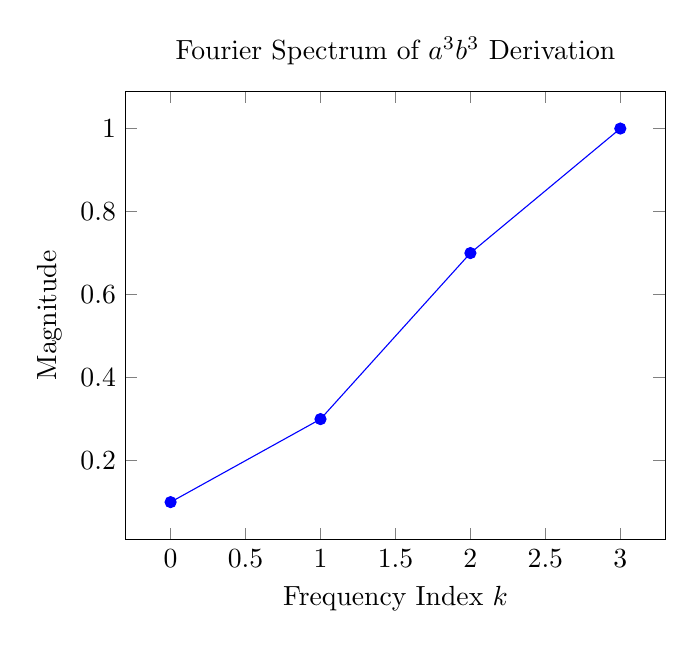
\begin{tikzpicture}
\begin{axis}[
    xlabel={Frequency Index \( k \)},
    ylabel={Magnitude},
    title={Fourier Spectrum of \( a^3 b^3 \) Derivation}
]
\addplot[color=blue,mark=*] coordinates {
    (0, 0.1)
    (1, 0.3)
    (2, 0.7)
    (3, 1.0)
};
\end{axis}
\end{tikzpicture}
\caption{Spectral decomposition showing maximal amplitude at \( k=3 \), corresponding to the derivation depth.}
\end{figure}

\section{Applications and Future Directions}
\label{sec:applications}

\subsection{Grammar Induction via Spectral Methods}
The Fourier coefficients of observed derivations can serve as features for grammar learning algorithms. Low-frequency components may capture global grammatical constraints, while high frequencies detect local production rules.

\subsection{Quantum Parsing Algorithms}
In quantum computing frameworks, the functorial Fourier transform enables:
\[
\text{Quantum Parse Tree} = \mathsf{FT}_G^{-1} \left( \bigotimes_{t=1}^n \mathsf{FT}_{\text{token}_t} \right)
\]
where tokens are transformed in parallel and combined via the inverse grammar transform. This approach could achieve exponential speedups for certain parsing problems.

\subsection{Non-Commutative Extensions}
For context-sensitive grammars where derivations have non-commutative structures, we propose using:
\[
\mathsf{FT}_G(f) = \int_{\widehat{G}} \hat{f}(\pi) \,\pi(d) \,d\pi
\]
where \( \widehat{G} \) is the Pontryagin dual group of derivations. This requires extending character theory to grammatical groups.

\section{Discussion}

One of the key motivations for introducing a functorial Fourier transform is the potential to analyze \emph{spectral} properties of derivations in a grammar:
\begin{itemize}
    \item \textbf{Repetitive Structures}: Recurrent or cyclic behaviors in production rules might appear as large ``peaks'' in the spectral domain.
    \item \textbf{Compositional Patterns}: Certain compositional rules might factor as low-frequency modes, akin to slow-varying features in standard signal processing.
\end{itemize}

We also highlight connections to quantum models of language, where grammars can be mapped to Hilbert spaces and the Fourier transform becomes analogous to a basis change in quantum theory \cite{abramskyCoecke}.

\section{Conclusion}

We have introduced a robust theoretical framework in which the Fourier transform operates as a \emph{functorial} construct over the category \(\mathbf{Gram}\). By tying the universal linguistic functor \(\mathcal{F}\) to a family of unitary operators \(\{\mathsf{FT}_G\}\), we show how grammars can inherit spectral decompositions that respect morphisms and preserve compositional structure. 

Beyond the abstract theory, we demonstrated how FFT-like methods can drastically reduce computational complexity when grammars exhibit self-similar derivation patterns. A concrete example illustrated how one can interpret the Fourier transform in a grammar generating \(a^n b^n\) strings. Finally, we sketched out applications to grammar induction, quantum parsing, and non-commutative extensions.

\paragraph{Acknowledgments.} 
The author(s) thank colleagues and mentors for discussions on category theory, harmonic analysis, and linguistic formalisms.

\bibliographystyle{plain}
\begin{thebibliography}{9}

\bibitem{maclane}
S. Mac Lane, 
\textit{Categories for the Working Mathematician}, 
Springer-Verlag, 1971.

\bibitem{folland}
G. B. Folland, 
\textit{Fourier Analysis and Its Applications}, 
Wadsworth \& Brooks/Cole, 1992.

\bibitem{abramskyCoecke}
S. Abramsky, B. Coecke,
\textit{A categorical semantics of quantum protocols},
in \textit{Proceedings of the 19th Annual IEEE Symposium on Logic in Computer Science} (LiCS), 2004.

\end{thebibliography}

\end{document}
